\documentclass[12pt]{article}
\usepackage[utf8]{inputenc}
\usepackage{graphicx}
\usepackage{amsmath}
\usepackage{hyperref}
\usepackage{xcolor}
\hypersetup{
    colorlinks=true,
    linkcolor=blue,
    filecolor=magenta,      
    urlcolor=blue,
    pdftitle={Overleaf Example},
    pdfpagemode=FullScreen,
    }

\begin{document}


\begin{titlepage}
\begin{center}
       \vspace*{1cm}

       \textbf{Detector-Encoder Autoencoders for Unsupervised Decomposition into Visual Parts}
       
       \vspace{1.5cm}

       Mohammad Sadil Khan\\M.Sc in Machine Learning and Data Mining\\
       \textbf{Supervisor:} Remi Emonet, Theirry Fournel, Amaury Habrard

       \vfill
            
       %\vspace{0.8cm}
            
       Hubert Curein Laboratory\\
       University Jean Monnet\\
       July 2,2021\\
       
\includegraphics[scale=4]{logo.png}
            
   \end{center}
\end{titlepage}


\newpage
\tableofcontents
\newpage

\section{Abstract}
\setcounter{page}{2}
In this project, we present a novel idea of using DAE, detecter-encoder autoencoders to detect anomaly in images, which will help decide whether some documents (thus the books) can be attributed to Marc-Michel Rey, a publisher of Thinkers. DAE is end-to-end trainable. We also introduce AutoLabelme, a graphical user interface and an extension of LabelMe, for efficiently and automatically annotating Images. We also present Ransac, a gui which can align some given images based on a reference image. The github code is available at \href{https://github.com/SadilKhan/internship-hubert-curien-2021}{https://github.com/SadilKhan/internship-hubert-curien-2021}
\section{Introduction}
\subsection{Lab Overview}
The Hubert Curien laboratory is a joint research unit (UMR 5516 ) of the Jean Monnet University, Saint-Etienne, the National Research Centre "CNRS" and the Institut d’Optique Graduate School. It is composed of about 90 researchers, professors and assistant professors, 20 engineers and administrative staff and 130 PhD and post-PhD students. This makes the Hubert Curien laboratory with a total of about 240 staff the most important research structure of Saint-Etienne. The research activities are organized according to two scientific departments: Optics, photonics and  surface and Computer Science, Security, Image.
\subsection{Internship Task}
The project is a part of ANR Roii (Rey's Ornament Image Investigation) researchers in the fields of the history of ideas, literature and the history of books (Ihrim) on the one hand, and computer vision and machine learning (Hubert Curien Laboratory) on the other.The aim of this collaborative and interdisciplinary project is to design a tool to help authenticate books published under fictitious or counterfeit names or addresses in the 18th century, through the analysis of ornaments.It is based on the design of a database of ornaments used by the bookseller Marc Michel Rey (1720-1780), the largest and most important publisher in the French language in the United Provinces.
The editorial and commercial practices of this French-speaking bookseller based in Amsterdam are indeed particularly representative of both the typographical uses of ornaments and the strategies for circumventing censorship. \\
The study of these editorial strategies is enlightening in order to understand the booktrade system and the way in which the sharing of knowledge and ideas on a European scale was practised at a time when it was beginning to be defended philosophically. These strategies make it particularly difficult to attribute a work to a publisher and to distinguish between genuine and counterfeit works. The investigation of ornaments then constitutes an additional clue to identify the works, within a cluster of concordant clues. The database is thus associated with an anomaly detection task, combining computer vision and automatic learning. A decision support tool was designed likely to reveal differences in shape at the level of wood ornaments and the publisher's mark, and differences in typographic style at the level of compound ornaments, based on the content of the database's data. \\
\textcolor{red}{CHECK$\downarrow$}\\
The rest of this report is organized as follows. Deep Learning requires huge set of training images. This paper discusses the methods the dataset is created in section 3. In section 4, the algorithms we used to create the network like SSD and Autoencoder are explained. In section 5 the approach for the novel method is discussed

\section{Graphical User Interface}
We introduce two graphical interfaces developed in Python for our project.
\begin{itemize}
    \item \textbf{AutoLabelMe}: Automatic Image Annotation
    \item \textbf{Ransac}: Image Alignment
\end{itemize}
\subsection{AutoLabelme}
\subsubsection{Introduction}
Data Collection is a major step in every Machine Learning projects. The quality and quantity of data alone can greatly impact the results of the model. Since we are at the beginning of the project, we had to devise a way to create a dataset for object detection purposes. We have 18 images and all the images are filled with vignettes/Components. Our first job was to create a bounding box around each and every object.\\
AutoLabelme is an automatic image annotator created using the Tkinter library in Python. It's an extension of LabelMe, the open-source Image Annotator available in \href{https://github.com/wkentaro/labelme}{https://github.com/wkentaro/labelme}. It matches the template provided by the user in an image and find same objects associating a bounding box and label for every object.
Autolabelme uses Normalized Cross-Correlation to check whether two templates are similar. It is designed keeping in mind with the necessity of creating dataset for object detection purposes and currently can only find objects in the cropped image i.e the search space to find same object is the space around the current template.
\subsubsection{Properties}
\begin{itemize}
    \item AutoLabelMe is simple to use. After LabelMe Manual Annotation just run AutoLabelMe.py.
    \item It is fast. We reduced the search space to the neighbourhood of the template which made it efficient for our given project.
    \item AutoLabelMe can identify rotated, scaled, horizontally and vertically flipped templates. There is no need for manually annotate rotated version of any template. It assigns a new label for the rotated templates with the rotaion information added in the label.
    \item AutoLabelMe also saces any meta information user stores during the LabelMe Manual Annotation step. For example, if for a bouding box, user assigns its label as "0 This is a Sun". AutoLabelMe will create a separate json file storing the new label for the bounding box and the meta information. This is helpful to save any additional information user wants for any object.
\end{itemize}

\begin{figure}[h]
    \centering
    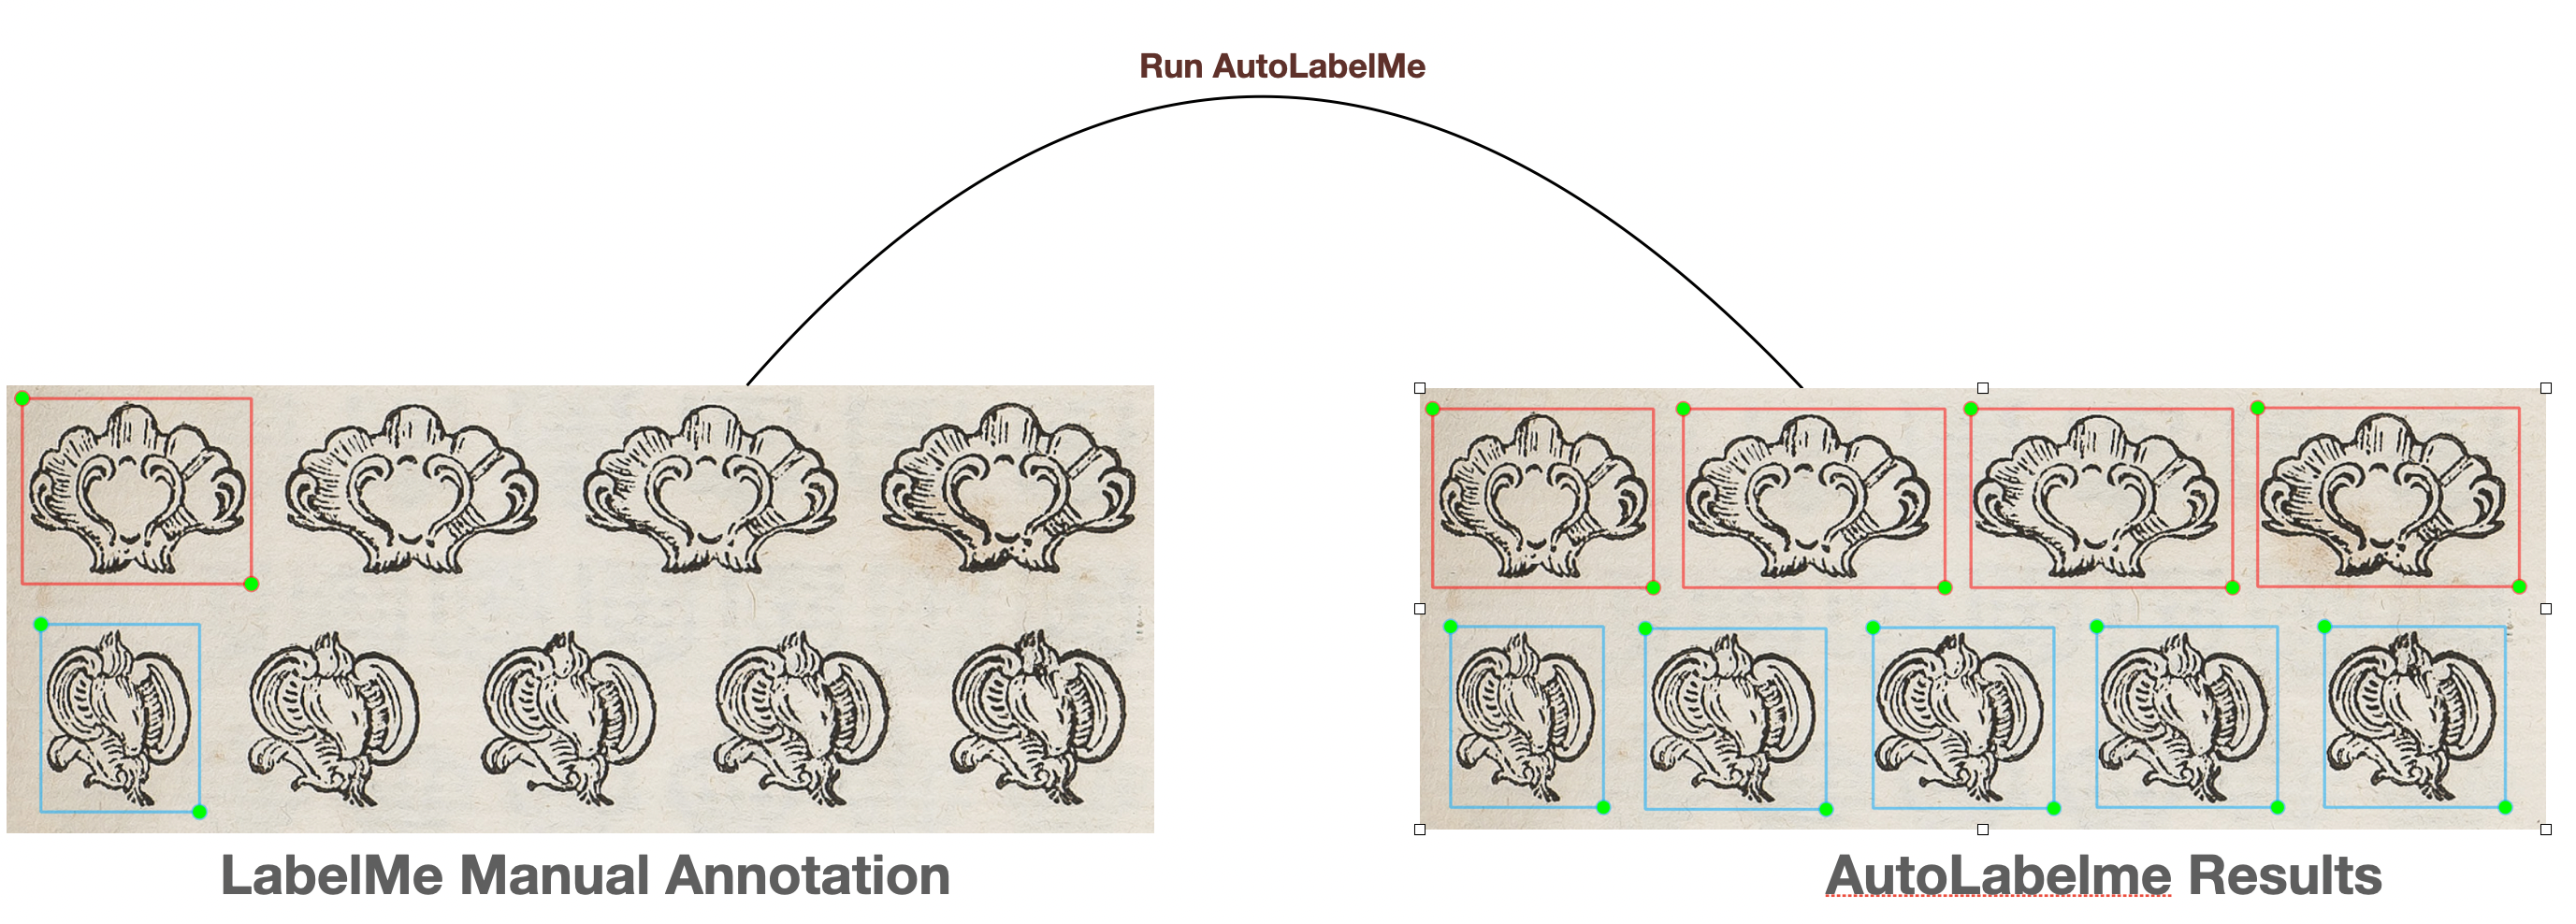
\includegraphics[scale=0.28]{Autolabelme results.png}
    \caption{Demonstration of autolabelme results}
    \label{fig:mesh1}
\end{figure}
\subsubsection{Tutorial}
\begin{figure}[h]
    \centering
    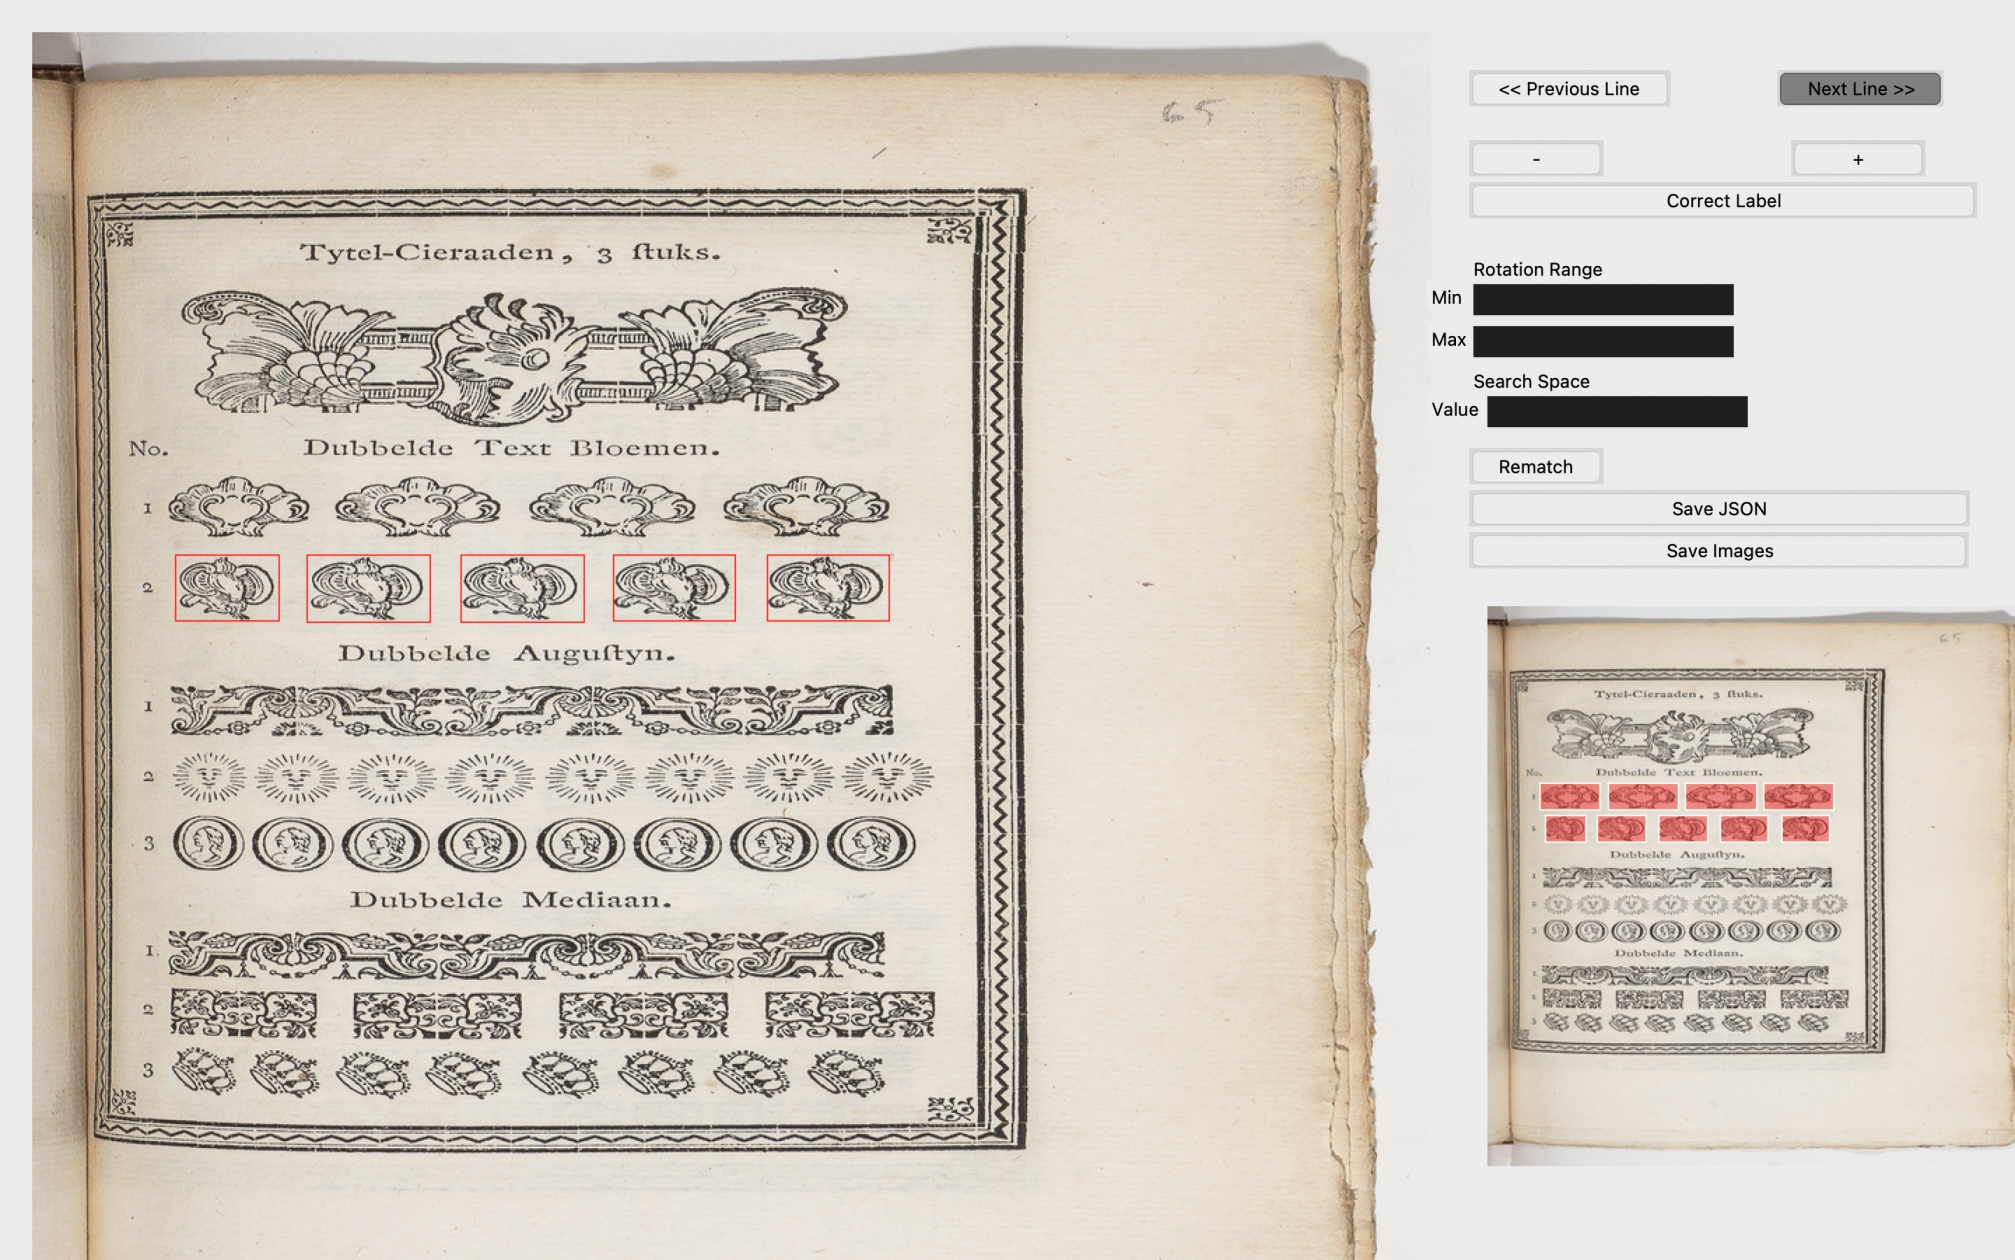
\includegraphics[scale=0.2]{View Autolabelme.jpg}
    \caption{Autolabelme Interface}
    \label{fig:mesh2}
\end{figure}
\begin{flushleft}
\textbf{Types of Windows}:\\
\end{flushleft}
1. \textit{Left Pane}: Shows the image and matching for the current label. \textcolor{red}{Red} for the usual boxes.\textcolor{blue}{Blue} for horizontally or vertically flipped boxes. \textcolor{green}{Green} for rotated. Although these are not final colors of the boxes. These are present only for checking.\\
2.\textit{Top-Right Pane}: Buttons.\\
3.\textit{Bottom-Right Pane}: Shows the image with all the matched templates. These image is helpful to recognise if every templates are matched or not. If any is missing, it can be added using LabelMe.\\[2em]
\textbf{Functions for every Button:-}\\
1.\textit{Next Line $>>$}: Template matching for next label.\\
2. \textit{$<<$ Previous Line}: Template Matching for the previous label.\\
3. $-$: Increases the threshold which results in less number of boxes.\\
4. $+$: Decreases the threshold which results in more number of boxes.\\
5. \textit{Save JSON}: Saves a JSON file which can be read by LabelMe for further edits.\\
6. \textit{Save Images}: Save the cropped vignettes from the image.\\
7. \textit{min}: The minimum value for Rotation.\\
8. \textit{max}: The maximum value for Rotation.\\
9. \textit{Rematch}: Match again for current label.\\
10. \textit{Correct Label}: Transform all the boxes to red boxes(no flip).\\[2em]
\textbf{How to Run:-}\\
1. Open Terminal.\\
2. Write \textit{labelme} or \textit{python3 /path/to/labelme.py}. Check \href {https://github.com/wkentaro/labelme}{https://github.com/wkentaro/labelme} for more details.\\
3. Create one bounding box per label.\\
4. Run AutoLabelme.py \textit{ python3 /path/to/AutoLabelme.py}.\\
5. Open JSON and press \textit{Next Line $>>$} to start matching.\\
6. The Left Image will show the boxes for current Label. The smaller right image is for showing all the templates.\\
7. Press \textit{$<<$ Previous Line} for viewing the matched boxes for the previous label.\\
8. Press $+$ for more boxes and $-$ for less boxes.\\
9. If you have rotated image, fill the rotation range or just enter \textit{min} value. For example \textit{min}=45 and \textit{max}=90 will give \textit{list(range(45,91,5))} values or just enter \textit{min}=45 which will only rotate the image once (45 degree).\\
10. The \textit{search space value} is by default 2 which means the algorithm will check for the templates from two heights up to two heights down in the original image. Choose any value from 1 to 15. For example if your template starts from coordinate (200,200) and height and width is 100 and 100 respectively and search space=2, the algorithm will search for the template from (0,0) to (400,400) in the image. If you select more than 15 than it's just \textit{heights-the value}. For example, if you choose 100 in the previous example, the it will be (0,100) to (300,300) where the templates will be searched in the image. In any case, value from 1 to 15 is sufficient.\\
11. Press \textit{Rematch} button or Press \textit{Enter} or \textit{Return} in your keyboard.\\
12.(Optional) Sometimes if the template is symmetric, the algorithm picks up some templates as flipped, to fix this, press \textit{Correct Label}.\\
13. Press  \textit{Save JSON} to save a json file.\\
14. Open the saved json file in Labelme. Labelme will show the matched templates. Edit it if necessary.\\
15. Press \textit{Save Images} in AutoLabelme if all the boxes are okay. This will save the matched templates in JPEG.\\[2em]


\subsection{Ransac}
\subsubsection{Introduction}
The images that are used are taken from books resulting in the projective transformation of the vignettes on the left side. To fix this we use Ransac-Flow\cite{ransac} (from \href{https://github.com/XiSHEN0220/RANSAC-Flow}{https://github.com/XiSHEN0220/RANSAC-Flow}). It's two-stage image-alignment process, first, a feature-based parametric coarse alignment using one or more homographies, followed by non-parametric fine pixel-wise alignment.Coarse alignment is performed using RANSAC on off-the-shelf deep features. Fine alignment is learned in an unsuper- vised way by a deep network which optimizes a standard structural similarity metric (SSIM) between the two images, plus cycle-consistency.\\
\subsubsection{Tutorial}
\begin{figure}[h]
    \centering
    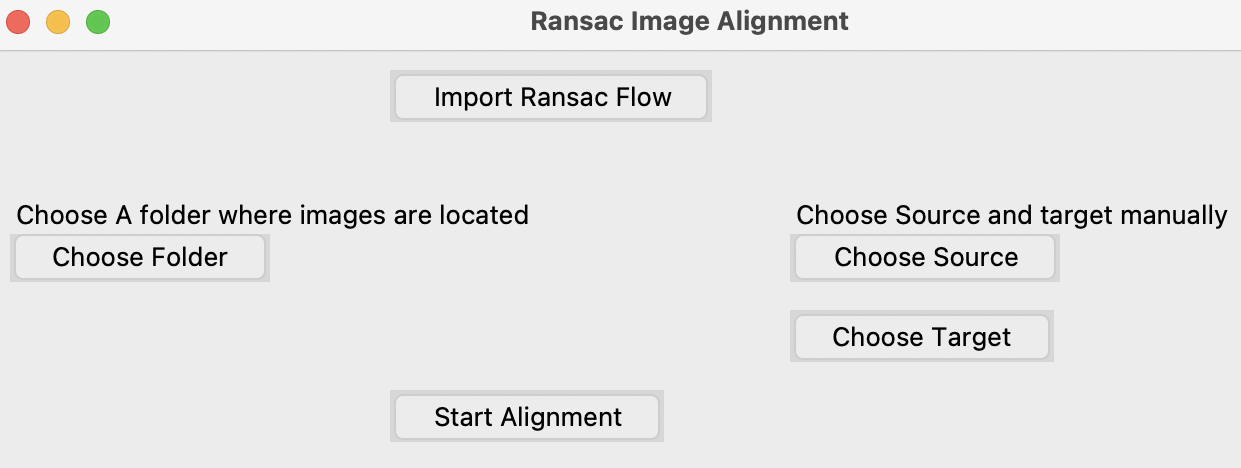
\includegraphics[scale=0.48]{Ransac Interface.png}
    \caption{Ransac Interface}
    \label{fig:mesh3}
\end{figure}
%\vspace{2em}
\begin{flushleft}
\textbf{Functions of Buttons:}\\
\end{flushleft}
1. \textit{Import Ransac Flow}: Opens Directory to import ransac flow python library.
2. Ransac Flow needs a Reference Image(Target) and a Source image for alignment.\\ There are two ways to import images in Ransac.
\begin{itemize}
    \item \textit{Choose Folder:} Choose the folder where the images are saved. The last image will be chosen as Reference and rest of them will be chosen as targets.
    \item \textit{Choose Target}: Choose the target image.\\
    \textit{Choose Source}: Choose manually the source image/images.
\end{itemize}
3. \textit{Start Alignment:} Choose which folder to save. The aligned images are saved.
\begin{figure}[h]
    \centering
    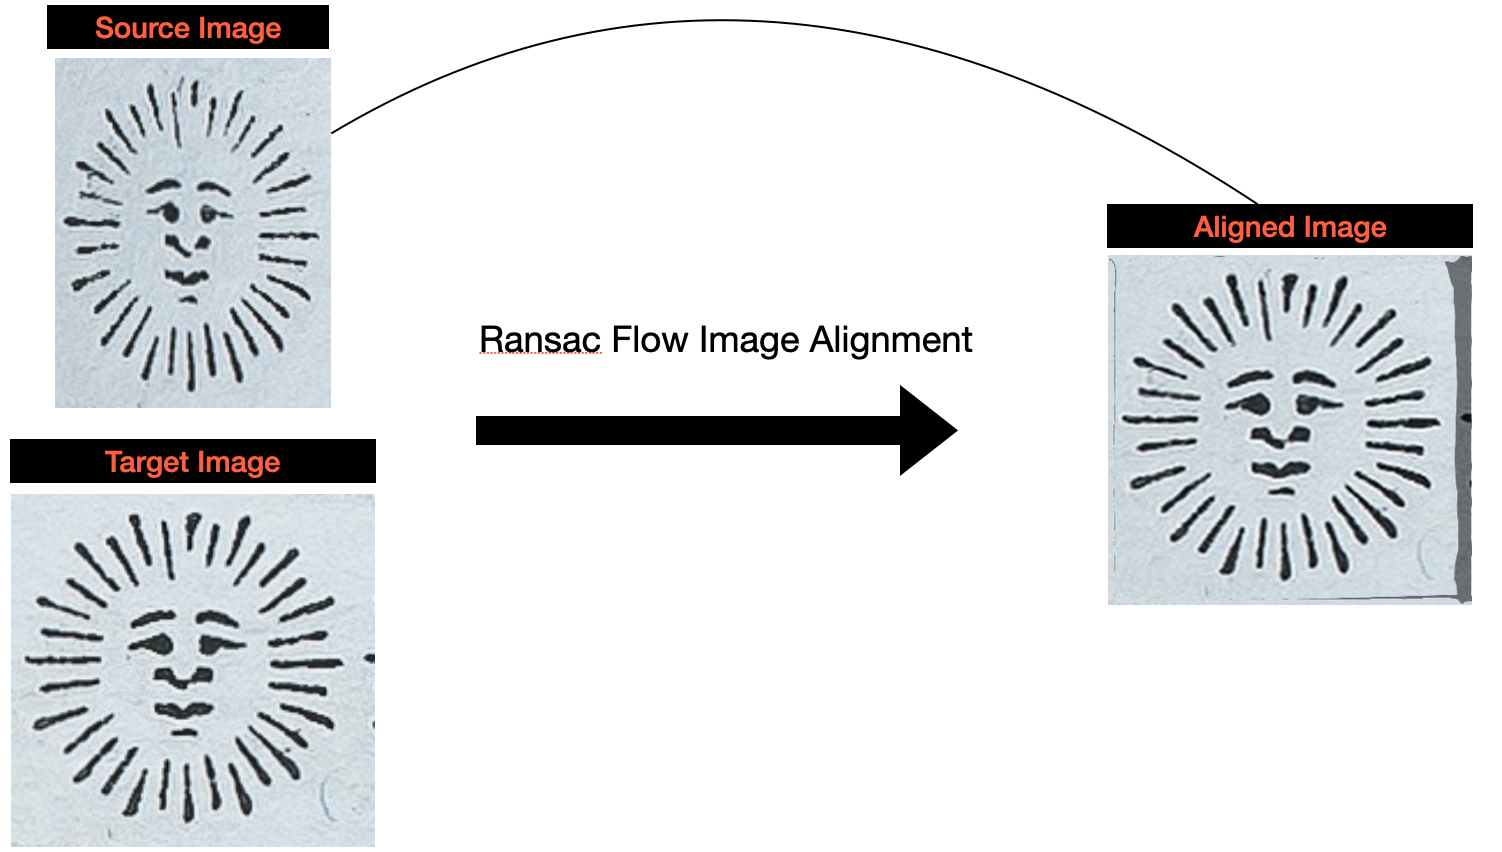
\includegraphics[scale=0.48]{Ransac Example.png}
    \caption{Example of Image alignment in Ransac}
    \label{fig:mesh4}
\end{figure}

\section{Models}
Our proposed method uses an object detector as an encoder and adds a decoder to construct an image. The objective is to recreate the image with the objects that are not in the catalogue as blurry. With this process we can detect the anomalies that will lead to any ornaments labelled as fraudulent. To achieve this task, our network should have the following properties:
\begin{itemize}
    \item The network should be end-to-end trainable which will be possible if the detector is end-to-end trainable.
    \item The detector needs to be fast and the predicted boxes should be precise. (High mean average precision).
\end{itemize}
Pre-existing domain-specific image object detectors usually
can be divided into two categories, the one is two-stage
detector, the most representative one, Faster R-CNN \cite{fasterrcnn}.
The other is one-stage detector, such as YOLO \cite{yolov1}, SSD\cite{ssd}.\\
Two-stage detectors have high localization and object
recognition accuracy, whereas the one-stage detectors achieve
high inference speed. The two stages of two-stage detectors
can be divided by RoI (Region of Interest) pooling layer.
For instance, in Faster R-CNN, the first stage, called RPN, a
Region Proposal Network, proposes candidate object bounding
boxes. The second stage, features are extracted by RoIPool
(RoI Pooling) operation from each candidate box for the following classification and bounding-box regression tasks. But two-stage detectors are not fully trainable. Although in FasterRCNN, RPN and FastRCNN can be jointly trained but it results in appoximate Furthermore, the one-stage detectors propose predicted boxes from input images directly without region proposal step, thus they are time efficient and can be used for real-time devices. So we proceed with SSD300 because of its speed and accuracy.\cite{survey}\\

\subsection{Single-Shot Multibox Detector(SSD)}
SSD is a single-shot object detector for multiple categories that is faster than the previous state-of-the-art for single shot detectors (YOLO), and significantly more accurate, in fact as accurate as slower techniques that perform explicit region proposals and pooling (including Faster R-CNN). SSD is end-to-end trainable and even on low resolution input images, it improves the speed vs accuracy trade-off. \\
The SSD approach is based on a feed-forward convolutional network that produces a fixed-size collection of bounding boxes and scores for the presence of object class instances in those boxes, followed by a non-maximum suppression step to produce the final detections. The early network layers are based on a standard architecture used for
high quality image classification (truncated before any classification layers), which is called the base network[Fig 5]. Auxiliary structures are added to the network to produce detections with the following features:-
\begin{figure}[h]
    \centering
    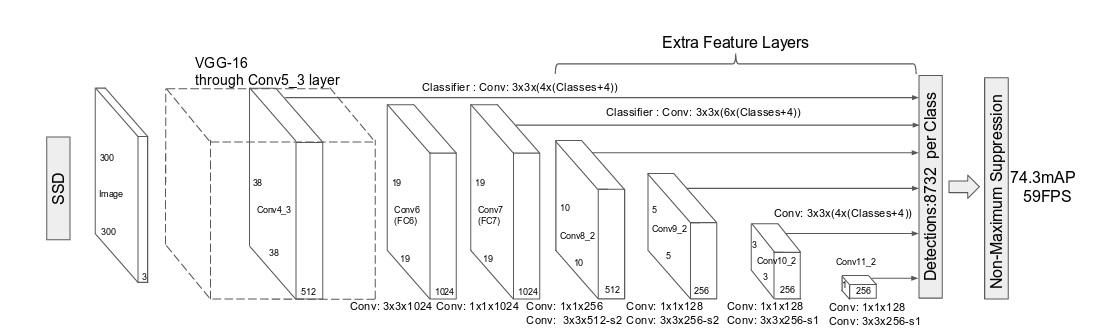
\includegraphics[scale=0.38]{ssd architecture.png}
    \caption{SSD architecture. Base network(vgg16) is truncated at conv5$\_$3 layer and auxiliary network is then added.}
    \label{fig:mesh5}
\end{figure}
\subsubsection{Multi-Scale Feature Maps}
Convolutional Layers are added to the base network which progressively decrease in size and allow predictions of different scales. In Figure 6, it can be seen that in lower layers bigger objects are captured more precisely and in the upper layers when the feature maps are large, the smaller objects are detected. For example, the following feature maps are selected for detection purposes.
\begin{itemize}
    \item \textbf{Conv4$\_$3:} Size $38\times 38\times 512$ 
    \item \textbf{Conv7:} Size $19\times 19\times 1024$ 
    \item \textbf{Conv8$\_$2:} Size $10\times 10\times 512$ 
    \item \textbf{Conv9$\_$2:} Size $5\times 5\times 256$ 
    \item \textbf{Conv10$\_$2:} Size $3\times 3\times 256$
    \item \textbf{Conv11$\_$2:} Size $1\times 1\times 256$ 

\end{itemize}
\subsubsection{Default Boxes}
For each of the feature maps, for each cell, SSD associates 4 or 6 boxes of different scale and aspect ratios[Figure 6] with objectness score. These are called default boxes which tile the feature map in a convolutional manner so that the position of each box relative to its corresponding cell is fixed. 
\begin{figure}[h]
    \centering
    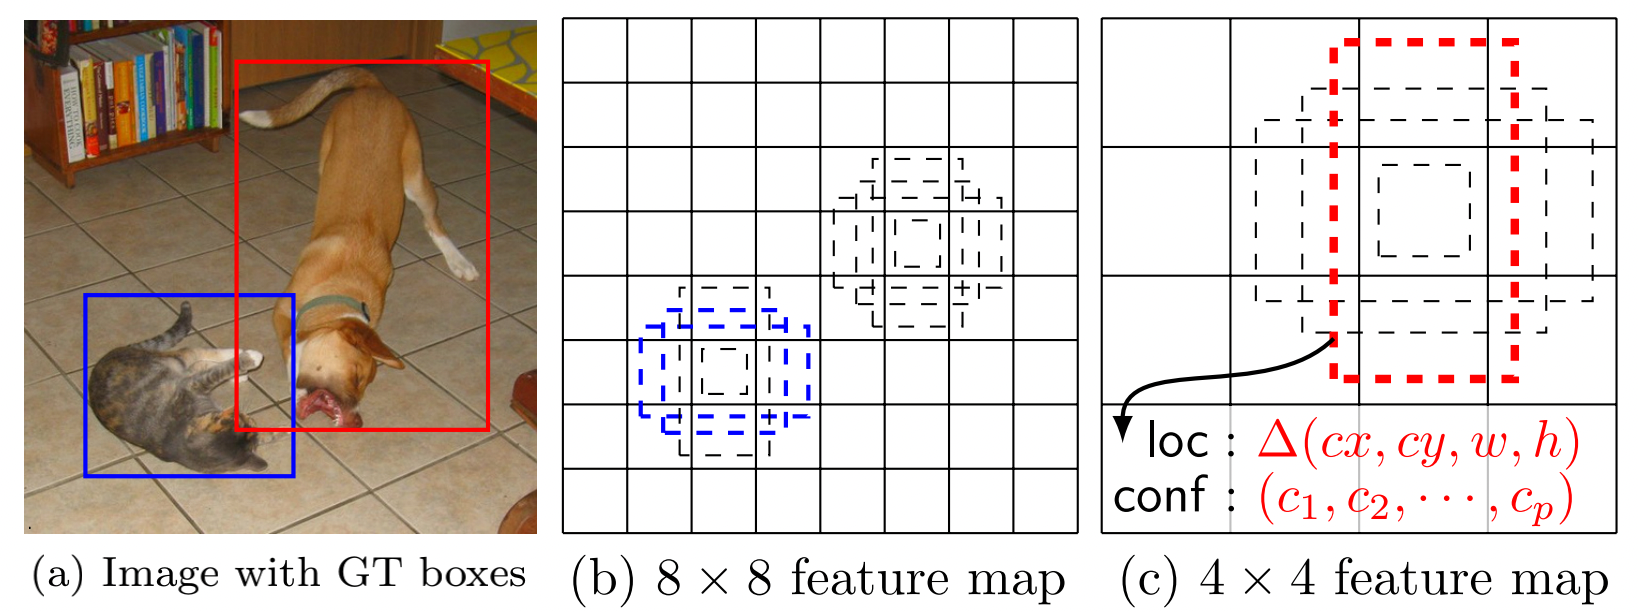
\includegraphics[scale=0.38]{Default Boxes.png}
    \caption{SSD. Default Boxes}
    \label{fig:mesh5}
\end{figure}\\
Default boundary boxes are chosen manually. SSD defines a scale value for each feature map layer. Starting from the left, Conv4$\_$3 detects objects at the smallest scale 0.1 (or 0.2 sometimes), and then increases linearly to the rightmost layer at a scale of 0.9. \\The scales for every layers are takes as follows:\\
\begin{itemize}
    \item \textbf{Conv4$\_$3:} 0.1
    \item \textbf{Conv7:} 0.2
    \item \textbf{Conv8$\_$2:} 0.375
    \item \textbf{Conv9$\_$2:} 0.55
    \item \textbf{Conv10$\_$2:} 0.725
    \item \textbf{Conv11$\_$2:} 0.9
\end{itemize}
Combining the scale value with the target aspect ratios, SSD compute the width and the height of the default boxes. For layers making 6 predictions, SSD starts with 5 target aspect ratios: 1, 2, 3, 1/2, and 1/3 and the layers making 4 predictions, 3 target aspect ratios 1,2,0.5. Then the width and the height of the default boxes are calculated as:\\
\begin{align*}
    & w=scale \times \sqrt{aspect\enspace ratio}\\
    & h=\frac{scale}{\sqrt{aspect\enspace ratio}}\\
\end{align*}
Then SSD adds an extra default box with scale\\
\begin{align*}
    scale=\begin{cases}
    \sqrt{scale\times \textit{scale at the next level}}\\
    1 \textit{ for the last level}
    \end{cases}
\end{align*}

Total number of default boxes $38\times 38 \times 4+19 \times 19 \times 6+10\times 10\times6+5\times5\times6+3\times3\times4+1\times1\times4$=8732.
For each one of the boxes $b_{ij}^{k}$ (the box associated with $(ij)th$ coordinate of the $kth$ feature map), SSD predicts offsets relative to the default box shapes in the cell and confidence score $P(c_{n}/b_{ij}^{k}) \quad \forall n=1,2...,num\_classes$ i.e the probability of object class $c_{n}$ in the box $b_{ij}^{k}$. Finally non-maximum suppression is performed to produce the final detection box.\\



\begin{flushleft}
\textbf{Matching Strategy}
\end{flushleft}
SSD predictions are classified as positive matches or negative matches. SSD only uses positive matches in calculating the localization cost (the mismatch of the boundary box). If the corresponding default boundary box (not the predicted boundary box) has an IoU greater than 0.5 with the ground truth, the match is positive. Otherwise, it is negative. (IoU, the intersection over the union, is the ratio between the intersected area over the joined area for two regions.)

\begin{figure}[h]
    \centering
    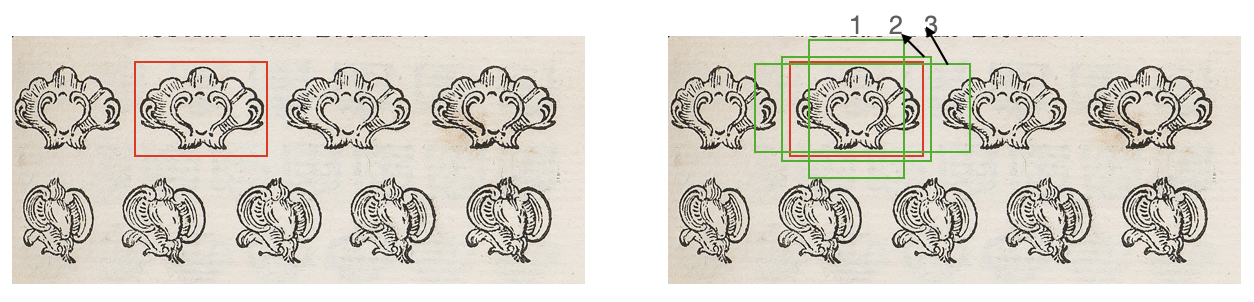
\includegraphics[scale=0.58]{ssd_default_ground.png}
    \caption{The ground truth box(red) and three default boxes(green)}
    \label{fig:mesh6}
\end{figure}

For example let's take 3 default boxes. Only default box 1 and 2 (but not 3) have an IoU greater than 0.75 with the ground truth box above (blue box). So only box 1 and 2 are positive matches. Once identify the positive matches are identified, corresponding predicted boundary boxes are used to calculate the cost. This matching strategy nicely partitions what shape of the ground truth that a prediction is responsible for. This matching strategy encourages each prediction to predict shapes closer to the corresponding default box. Therefore the predictions are more diverse and more stable in the training.





\subsubsection{Loss Function}
SSD has two loss functions:- Localization Loss and Classification Loss
\begin{flushleft}
\textbf{Locatization Loss}
\end{flushleft}
The localization loss is the mismatch between the ground truth box and the predicted boundary box. SSD only penalizes predictions from positive matches. Since the predictions from the positive matches are desired to get closer to the ground truth. Negative matches can be ignored.\\
The locatization loss between the predicted box l and the ground truth box g is defined as the smooth l1 loss with cx,cy as the offset to the default bounding box d of width w and height h.
\begin{align*}
    & \text{Let } O=\{cx,cy,w,h\} \\
    & L_{loc}(x,l,g)=\sum_{i\in Pos}^{N} \sum_{m\in O} x_{ij}^{k} smooth_{L1}(l_{i}^{m}-\hat{g}_{j}^{m})\\
    & \hat{g}_{j}^{cx}=(g_{j}^{cx}-d_{i}^{cx})/d_{i}^{w}, \hat{g}_{j}^{cy}=(g_{j}^{cy}-d_{i}^{cy})/d_{i}^{h}.\\
    & \hat{g}_{j}^{w}=log(\frac{g_{j}^{w}}{d_{i}^{w}}), 
    \hat{g}_{j}^{h}=log(\frac{g_{j}^{h}}{d_{i}^{h}})
\end{align*}
\begin{align*}
x_{ij}^{p}=
    \begin{cases}
    1 & \text{ if } IOU> 0.5 \text{ between default box i and ground truth box j on class p}\\
    0 & Otherwise
    \end{cases}
\end{align*}

\begin{flushleft}
\textbf{Confidence Loss}
\end{flushleft}
The confidence loss is the loss of making a class prediction. For every positive match prediction, we penalize the loss according to the confidence score of the corresponding class. For negative match predictions, we penalize the loss according to the confidence score of the class “0”: class “0” classifies no object is detected.\\
It's calculated as the softmax loss over multiple classes confidences c(class score)\\
\begin{align*}
    & L_{conf}(x,c)=-\sum_{i\in Pos}^{N} x_{ij}^{k}log(\hat{c_{i}}^{p})-\sum_{i\in Neg}^{N} x_{ij}^{k}log(\hat{c_{i}}^{0})\\
    & where \enspace \hat{c_{i}}^{p}=\frac{exp(c_{i}^{p})}{\sum_{p}exp(c_{i}^{p})} \\
    & N \text{ is the Number of matched default boxes.}
\end{align*}
Finally, the SSD loss =
\begin{align*}
    L_{ssd}(x,c,l,g)=\frac{1}{N}(L_{conf}(x,c)+\alpha L_{loc}(x,l,g))
\end{align*}

\begin{flushleft}
\textbf{Hard Mining}
\end{flushleft}
However, SSD makes far more predictions than the number of objects present. So there are many more negative matches than positive matches. This creates a class imbalance that hurts training. The SSD model is trained to learn background space rather than detecting objects. However, SSD still requires negative sampling so it can learn what constitutes a bad prediction. So, instead of using all the negatives, we sort those negatives by their calculated confidence loss. SSD picks the negatives with the top loss and makes sure the ratio between the picked negatives and positives is at most 3:1. This leads to faster and more stable training.\\

SSD makes many predictions (8732) for better coverage of location, scale, and aspect ratios, more than many other detection methods. However, many predictions contain no object. Therefore, any predictions with class confidence scores lower than 0.2 will be eliminated.\\

\begin{figure}[h]
    \centering
    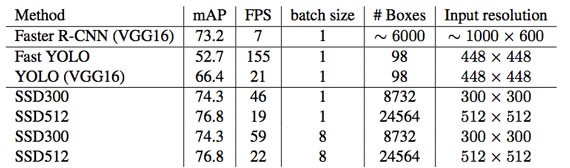
\includegraphics[scale=0.58]{inference_time.jpeg}
    \caption{Results of various detections.SSD makes more predictions. Improvements allow SSD to use lower resolution images for similar accuracy.}
    \label{fig:mesh6}
\end{figure}
\begin{flushleft}
\textbf{Non-Max Suppression}
\end{flushleft}
SSD uses non-maximum suppression to remove duplicate predictions pointing to the same object. SSD sorts the predictions by the confidence scores. Start from the top confidence prediction, SSD evaluates whether any previously predicted boundary boxes have an IoU higher than 0.45 with the current prediction for the same class. If found, the current prediction will be ignored. At most, top 200 predictions per image are kept.



\subsection{GIOU optimized SSD}
Bounding box regression is one of the most fundamental components in many 2D/3D computer vision tasks. Tasks such as object localization, multiple object detection, object tracking and instance level segmentation rely on accurate bounding box regression. The dominant trend for improving performance of applications utilizing deep neural networks is to propose either a better architecture backbone or a better strategy to extract reliable local features. However, one opportunity for improvement that is widely ignored is the replacement of the surrogate regression losses such as $l_{1}$ and $l_{2}$-norms, with a metric loss calculated based on Intersection over Union (IoU).IoU , also known as Jaccard index, is the most commonly used metric for comparing the similarity between two arbitrary shapes. IoU encodes the shape properties of the objects under comparison, e.g. the widths, heights and locations of two bounding boxes, into the region property and then calculates a normalized measure that focuses on their areas (or volumes). This property makes IoU invariant to the scale of the problem under consideration. Due to this appealing property, all performance measures used to evaluate for segmentation, object detection, and tracking rely on this metric.\cite{survey loss}\\

\begin{figure}[h]
    \centering
    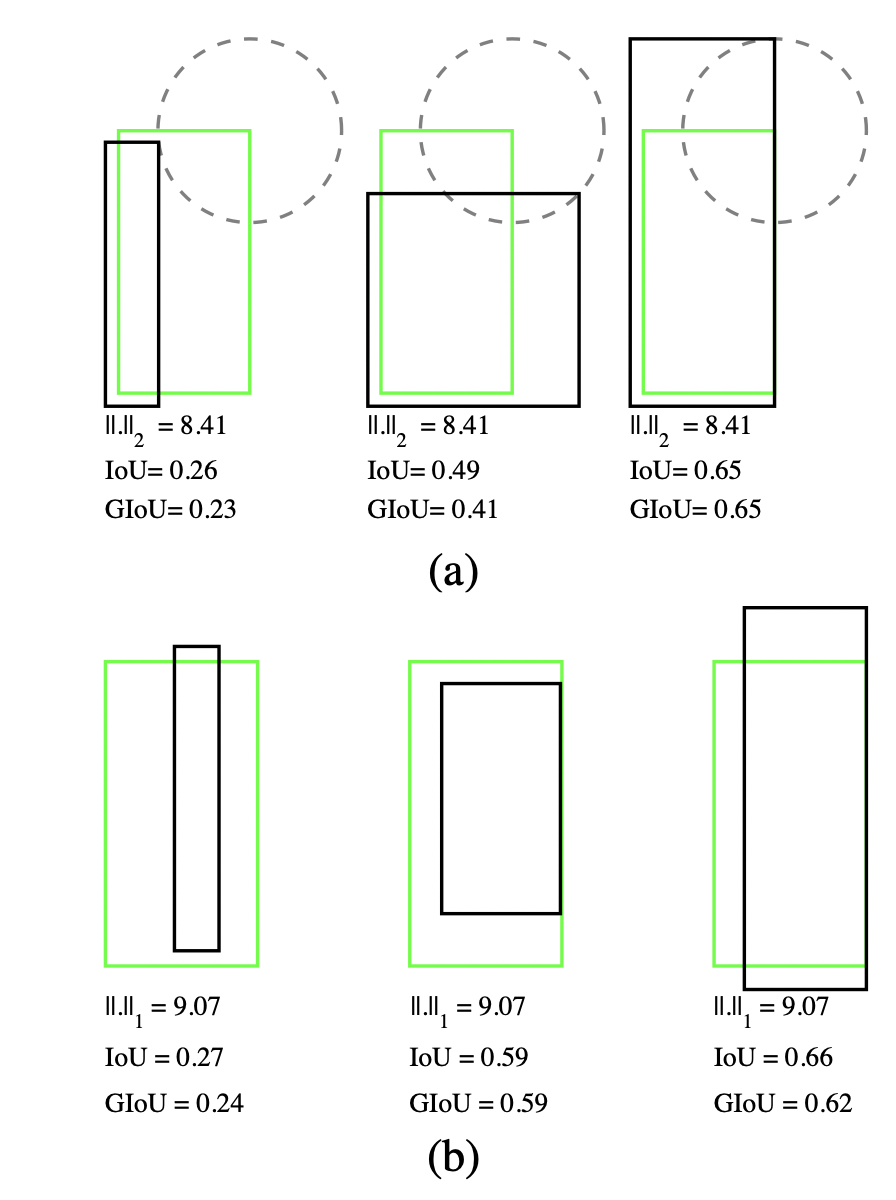
\includegraphics[scale=0.50]{l1_loss.png}
    \caption{Two sets of examples (a) and (b) with the bounding boxes represented by (a) two corners $(x_{1} , y_{1} , x_{2} , y_{2} )$ and (b) center and size $(x_{c}, y_{c}, w, h)$. For all three cases in each set (a) $l_{2}$- norm distance, $||.||_{2}$, and (b) $l_{1}$-norm distance, $||.||_{1}$, between the representation of two rectangles are exactly same value, but their IoU and GIoU values are very different.
}
    \label{fig:mesh6}
\end{figure}

However, it can be shown that there is not a strong correlation between minimizing the commonly used losses, e.g. $l_{n}-norms$, defined on parametric representation of two bounding boxes in 2D/3D and improving their IoU values. For example, consider the simple 2D scenario in Figure. 9 (a), where the predicted bounding box (black rectangle), and the ground truth box (green rectangle), are represented by their top-left and bottom-right corners, i.e. $(x_{1} , y_{1} , x_{2} , y_{2} )$. For simplicity, let’s assume that the distance, e.g. l2-norm, between one of the corners of two boxes is fixed. Therefore any predicted bounding box where the second corner lies on a circle with a fixed radius centered on the second corner of the green rectangle (shown by a gray dashed line cir- cle) will have exactly the same $l_{2}$-norm distance from the ground truth box; however their IoU values can be significantly different (Figure. 9 (a)). The same argument can be ex- tended to any other representation and loss, e.g. Figure. 9 (b). It is intuitive that a good local optimum for these types of objectives may not necessarily be a local optimum for IoU. Moreover, in contrast to IoU , $l_{n}$ -norm objectives defined based on the aforementioned parametric representations are not invariant to the scale of the problem. To this end, several pairs of bounding boxes with the same level of overlap, but different scales due to e.g. perspective, will have different objective values. In addition, some representations may suffer from lack of regularization between the different types of parameters used for the representation. For example, in the center and size representation, $(x_{c}, y_{c})$ is defined on the location space while (w, h) belongs to the size space. Complexity increases as more parameters are incorporated, e.g. rotation, or when adding more dimensions to the problem. To alleviate some of the aforementioned problems, state-of- the-art object detectors introduce the concept of an anchor box as a hypothetically good initial guess. They also define a non-linear representation to naively compensate for the scale changes. Even with these handcrafted changes, there is still a gap between optimizing the regression losses and IoU values.
\subsubsection{IOU Loss}
Generally, for two finite sample sets A and B, their IoU is defined as the intersection $(A \cap B)$ divided by the union $(A \cup B)$ of A and B.
\begin{align*}
    IoU(A,B)=\frac{|A \cap B|}{|A \cup B|}=\frac{|A \cap B|}{|A|+|B|-|A \cup B|}
\end{align*}
For bounding box-level object detection, the target object is usually represented by a minimum Bbox rectangle in the 2D image. Base on this representation, the IoU computation between the ground bounding box $B_{g}=(x_{1} , y_{1} , x_{2} , y_{2} )$ and the predicted bounding box $B_{d}=(x_{1}^{\prime} , y_{1}^{\prime} , x_{2}^{\prime} , y_{2}^{\prime} )$ is defined as:-
\begin{align*}
    & IoU(A,B)=\frac{\text{Area of overlap between $B_{g}$ and $B_{d}$}}{\text{Area of union of $B_{g}$ and $B_{d}$}}=\\ 
    & \frac{(max(x_{1},x_{1}^{\prime})-min(x_{2},x_{2}^{\prime}))\times (max(y_{1},y_{1}^{\prime})-min(y_{2},y_{2}^{\prime}))}{(x_{2}-x_{1}) (y_{2}-y_{1})+(x_{2}^{\prime}-x_{1}^{\prime}) (y_{2}^{\prime}-y_{1}^{\prime})-(max(x_{1},x_{1}^{\prime})-min(x_{2},x_{2}^{\prime})) (max(y_{1},y_{1}^{\prime})-min(y_{2},y_{2}^{\prime}))}
\end{align*}
Usually, objects are labeled with axis-aligned BBoxes in the ROI dataset. By taking this kind of labels as ground truth, the predicted BBoxes are also axis-aligned rectangles. For this case, the IoU computation is very easy.

\begin{flushleft}
\textbf{Loss function}:
\end{flushleft}
The IOU loss function\cite{iou} for the ground bounding box $B_{g}=(x_{1} , y_{1} , x_{2} , y_{2} )$ and the predicted bounding box $B_{d}=(x_{1}^{\prime} , y_{1}^{\prime} , x_{2}^{\prime} , y_{2}^{\prime} )$ is defined as
\begin{align*}
    L_{IoU}=1-IoU(B_{g},B_{d})
\end{align*}
\begin{itemize}
    \item Since $0\leq IoU \leq 1, 0\leq L_{IoU} \leq 1$. So $L_{IoU}$ is non-negative. $L_{IoU}=0 \text{ when } IoU(A,B)=1 \implies A=B$.
    \item $IoU(A,B)=IoU(B,A) \implies L_{IoU}(A,B)=L_{IoU}(B,A)$. So $L_{IoU}$ is symmetric.
    \item $L_{IoU}$ satisfies triangle inequality.\cite{iou_te}
\end{itemize}
So $L_{IoU}$ is a metric by mathematical definition.

\subsubsection{GIOU Loss}

\subsubsection{Results}
\subsection{AutoEncoder}
\section{Contribution}
\subsubsection{Data Preparation}
\subsubsection{Training SSD}
\subsubsection{Decoder-Detector}
\section{Future Work}
Patch detection and auto-encoding will be developed to be confronted or combined in order to deliver tangible visual elements on demand, with patch analysis approximating the mechanisms implemented during a visual comparison of facing images, the auto-encoders producing an efficient representation of the data in unsupervised mode. This tool will be blindly tested on collections of ornamental images attributed to Marc Michel Rey, but also on fakes recognized by experts, before being tested online and in open access, and eventually transferred from Marc Michel Rey's collection to other heritage collections.
\section{Conclusions}

\begin{thebibliography}{9}
\bibitem{ransac} 
Xi Shen, François Darmon, Alexei A. Efros, Mathieu Aubry.
\textit{\href{https://arxiv.org/abs/2004.01526}{RANSAC-Flow: generic two-stage image alignment.}}.

\bibitem{fasterrcnn} 
Shaoqing Ren, Kaiming He, Ross Girshick, Jian Sun.
\textit{\href{https://arxiv.org/abs/1506.01497}{Faster R-CNN: Towards Real-Time Object Detection with Region Proposal Networks.}}

\bibitem{ssd} 
Wei Liu, Dragomir Anguelov, Dumitru Erhan, Christian Szegedy, Scott Reed, Cheng-Yang Fu, Alexander C. Berg.
\textit{\href{https://arxiv.org/abs/1512.02325}{SSD: Singe Shot Detector.}}

\bibitem{yolov1} 
Joseph Redmon, Santosh Divvala, Ross Girshick, Ali Farhadi.
\textit{\href{https://arxiv.org/abs/1506.02640}{You Only Look Once: Unified, Real-Time Object Detection.}}

\bibitem{yolov2} 
Joseph Redmon, Ali Farhadi.
\textit{\href{https://arxiv.org/abs/1612.08242}{YOLO9000: Better, Faster, Stronger.}}

\bibitem{giou} 
Hamid Rezatofighi, Nathan Tsoi, JunYoung Gwak, Amir Sadeghian, Ian Reid, Silvio Savarese.
\textit{\href{https://arxiv.org/abs/1902.09630}{Generalized Intersection over Union: A Metric and A Loss for Bounding Box Regression.}}

\bibitem{iou} 
Dingfu Zhou, Jin Fang, Xibin Song, Chenye Guan, Junbo Yin, Yuchao Dai, Ruigang Yang
\textit{\href{https://arxiv.org/abs/1908.03851}{IoU Loss for 2D/3D Object Detection
}}
\bibitem{iou_te} 
Sven Kosub
\textit{\href{https://arxiv.org/pdf/1612.02696.pdf
}{A note on the triangle inequality for the Jaccard distance}}


\bibitem{survey loss} 
Yuanzhou Yao, Yuhang Yang, Xinyue Su, Yihang Zhao, Ao Feng, Yiting Huang, Haibo Pu
\textit{\href{https://www.atlantis-press.com/proceedings/iccia-19/125913142}{Optimization of the Bounding Box Regression Process of SSD Model
}}
\bibitem{maskrcnn} 
Kaiming He, Georgia Gkioxari, Piotr Dollár, Ross Girshick.
\textit{\href{https://arxiv.org/pdf/1703.06870.pdf}{Mask RCNN.}}

\bibitem{survey} 
Licheng Jiao, Fellow, IEEE, Fan Zhang, Fang Liu, Senior Member, IEEE, Shuyuan Yang, Senior Member, IEEE, Lingling Li, Member, IEEE, Zhixi Feng, Member, IEEE, and Rong Qu, Senior Member, IEEE.
\textit{\href{https://arxiv.org/pdf/1907.09408.pdf}{A Survey of Deep Learning-based Object Detection.
}}

\bibitem{blog1} 
\textit{\href{https://jonathan-hui.medium.com/ssd-object-detection-single-shot-multibox-detector-for-real-time-processing-9bd8deac0e06}{SSD object detection: Single Shot MultiBox Detector for real-time processing.
}}

\end{thebibliography}

\end{document}
